\documentclass[12pt, onecolumn]{IEEEtran}
\usepackage{cite}
\usepackage{amsmath,amssymb,amsfonts}
\usepackage{graphicx}
\usepackage{textcomp}
\usepackage{xcolor}
\usepackage{booktabs}
\usepackage{array}
\usepackage{url}
\usepackage{tikz}
\usetikzlibrary{shapes.geometric,arrows.meta,positioning}
\usepackage{setspace}
\usepackage{lineno}
\usepackage{geometry}
\geometry{a4paper, margin=2.5cm}

\begin{document}
\linenumbers
\doublespacing

\title{An Offline Multilingual Spoken Language Processing Pipeline for Indian Border Region Low-Resource Languages}

\author{Anonymous}

\maketitle

\begin{abstract}
Automatic speech recognition across India's contested border frontiers---the Line of Control with Pakistan (Punjabi, Urdu), the open border with Nepal (Nepali, Hindi), and the Sino-Indian Line of Actual Control (Mandarin Chinese)---requires handling languages that most large models have barely seen. On a typical Punjabi recording, Whisper returns Hindi: the two languages share the bulk of their phoneme inventory, and Punjabi has minimal presence in Whisper's 680,000-hour training corpus. The model does not fail noisily---it outputs a confident wrong answer that propagates through translation and summarisation without any warning to the operator. VANI (Voice Analysis and Neural Intelligence) is a fully offline, CPU-only, ten-stage spoken language processing pipeline built specifically to catch and correct this failure class across all five border-region language groups, requiring no Internet connection or GPU hardware. The core is a three-source language identification ensemble: Whisper encoder probability, FastText character n-gram scores, and MMS-LID-256 raw-audio predictions are fused under a confidence-weighted vote with Unicode script-block overrides for Gurmukhi and Arabic/Nastaliq script families. A five-language ablation study across 500 FLEURS test samples---Hindi, Punjabi, Urdu, Nepali, and Mandarin Chinese---traced the contribution of each component: adding MMS-LID raised the macro-average LangID accuracy from 50.8\% to 70.2\% (+19.4~pp), recovering Punjabi identification from 0\% to 89\% solely through audio-based evidence. The integrated pipeline achieves 81.7\% LangID accuracy across four Indic languages (70.0\% in the stricter ablation with \texttt{language\_hint=None}; see Section~\ref{sec:ablation}) and 100\% translation completion rate, running end-to-end on a consumer laptop within an edge-constrained memory budget.
\end{abstract}

\begin{IEEEkeywords}
Automatic speech recognition, Indian border region languages, Indic languages, spoken language processing, language identification, offline deployment, border security, Whisper, NLLB-200, MMS-LID, speaker diarisation, automated summarisation.
\end{IEEEkeywords}

\section{Introduction}
\label{sec:intro}

India's land borders trace three geopolitically distinct arcs that together span the full breadth of South and East Asia's linguistic diversity, as follows: The western arc---the Line of Control with Pakistan and the international boundary with Afghanistan---is dominated by Punjabi, Urdu, and Pashto. The northern arc, running through the open borders with Nepal and Bhutan, adds Nepali and Hindi. The eastern arc, along the Sino-Indian Line of Actual Control and the Myanmar frontier, brings Mandarin and Burmese into the operational picture. Each language family has its own script, phoneme inventory, and degree of representation in the datasets on which large ASR models were trained. Punjabi, Urdu, Nepali, and Mandarin Chinese are all under-resourced relative to the scale at which Whisper~\cite{radford2022whisper} and similar models were trained; the practical consequence is that field speech from these border regions is systematically misidentified and misrouted by off-the-shelf systems.

This broader challenge compounds the under-resourcing problem. Hindi, Punjabi, Urdu, Nepali, Dogri, Kashmiri, Pashto, and Sindhi are routinely encountered within the same geographic corridor, often code-switched within a single recording, and captured under adverse channel conditions. Field-recorded border audio typically arrives with bandwidth-limited channels, background static, and no guarantee that any predictable language boundary will be respected by the speaker.

The direct consequence of automated spoken language analysis is that off-the-shelf ASR pipelines fail in ways that are silent and difficult to detect. During development, we observed Whisper large-v3-turbo~\cite{radford2022whisper} returning a Hindi language probability of 0.707 on a recording where the speaker's script was unambiguously Gurmukhi. The model did not malfunction because Punjabi and Hindi share a large phoneme inventory, and Punjabi has far fewer training hours in Whisper's corpus. However, the downstream effect is straightforward: the recording is routed to Hindi translation, the operator sees plausible output with no warning, and the error is invisible unless the operator happens to know Punjabi. This is the failure mode for which the system was designed to close.

VANI addresses this by combining three independent identification signals---Whisper encoder probability, FastText text-based LangID, and MMS-LID-256 raw-audio LangID---under a confidence-weighted vote with hard Unicode script overrides. Speaker diarisation runs before language routing to attribute each segment to a speaker. A structured summarisation module converts the translated output into a 5\,W intelligence report with severity classification. The whole system runs offline on commodity edge hardware; models are loaded one at a time and explicitly released before the next stage to stay within the 8~GB RAM budget.

This study makes six contributions.
\begin{enumerate}
\item A modular ten-stage pipeline was evaluated at two scales: 120 samples across four Indic languages in the integrated pipeline evaluation and 500 samples across five languages from FLEURS (adding Mandarin Chinese) in the controlled ablation, all on a CPU-only edge-class device with no internet access.
\item A three-source LangID ensemble achieved 96.7\% accuracy for Hindi and Punjabi in the integrated pipeline evaluation, with detailed failure analysis for Urdu (70.0\%) and Nepali (63.3\%).
\item A five-language, four-configuration ablation study (Hindi, Punjabi, Urdu, Nepali, Mandarin; 500 samples total, FLEURS test split) quantifying each component's marginal gain: Whisper-only 49.0\% $\rightarrow$ +FastText 50.8\% $\rightarrow$ +MMS-LID 70.2\% $\rightarrow$ Full VANI 70.0\% (macro-averaged over five languages).
\item Evidence that audio-based MMS-LID is the single most important component for low-resource languages, adding +19.4~pp macro-average (50.8\%$\rightarrow$70.2\%)---the decisive step in the ablation---recovering Punjabi identification from 0.0\% to 89.0\% and Nepali from 0.0\% to 18.0\%.
\item A memory-efficient speaker diarisation stage using MFCC-based agglomerative clustering that enables per-speaker transcript attribution without any pre-trained speaker embedding model, while keeping the peak RAM within the edge-device budget during the active ASR pass. The next planned evaluation step is the diarisation error rate (DER) evaluation on standard annotated multi-speaker corpora.
\item A structured summarisation (SSUM) module that combines rule-based 5\,W extraction with an optional quantised LLM layer, producing structured reports with severity classification and upstream confidence flags.
\end{enumerate}

\section{Background and Related Work}

The practical landscape for multilingual speech processing shifted substantially in 2023. Whisper~\cite{radford2022whisper}, trained on 680,000~h of weakly supervised audio from 99 languages, established zero-shot multilingual transcription as a reliable capability for well-resourced languages---not merely a benchmark result. The MMS project~\cite{pratap2023scaling} extended coverage to 1,107 languages by training on a large corpus of audio from religious speech sources; its language identification component---the MMS-LID model used in this work---achieves over 90\% top-1 accuracy across 256 audio-only language classes by operating directly on raw waveforms rather than transcripts. Both systems confirmed the same pattern: accuracy was strong where training data were plentiful and degraded sharply for languages with limited representation, which is the operating condition for most of the target languages in this study.

For translation, NLLB-200~\cite{costajussa2024nllb} covers over 200 languages in a single shared model, including 21 of India's 22 constitutionally scheduled languages. Its distilled 600M-parameter variant fits within a constrained edge-deployment memory budget---the practical reason for choosing it over larger alternatives. Meta's SeamlessM4T~\cite{barrault2023seamless} subsequently unified speech recognition, translation, and speech synthesis across 100 languages into a single end-to-end framework. For this application a modular pipeline is the practical choice: loading one component at a time and measuring its RAM peak before releasing it gives fine-grained memory control that a monolithic end-to-end model does not easily allow on a constrained device.

FLEURS~\cite{conneau2023fleurs} provides the standardised evaluation framework used throughout this work: 102-language test splits drawn from read speech, enabling reproducible comparison across systems. A complementary benchmark, ML-SUPERB~\cite{shi2023mlsuperb}, evaluates multilingual speech understanding across 143 languages and shares FLEURS' goal of reproducible cross-system comparison; together they represent the current standard for evaluating coverage and accuracy at scale. The five languages evaluated in this study---Punjabi, Hindi, Urdu, Nepali, and Mandarin Chinese---were chosen specifically because they correspond to the five primary linguistic zones of India's contested borders. Mandarin Chinese is included not as a peripheral control language but as an operationally relevant target: PLA communications along the Line of Actual Control use Mandarin, and a pipeline that cannot identify Mandarin speech correctly cannot serve the northeastern theatre. Code-switching between Indic languages and English---and between Indic languages themselves---remains a challenging problem in the field. The phonological overlap between Punjabi and Hindi means that even high-quality recordings of Punjabi speech yield incorrect language predictions from systems trained primarily on Hindi-dominant corpora, a failure mode that FLEURS evaluation in this paper quantifies precisely.

Speaker diarisation, which involves assigning spoken segments to individual speakers, has advanced substantially in recent years through end-to-end neural systems~\cite{plaquet2023powerset} that now achieve single-digit diarisation error rates on clean multi-party audio. The practical constraint for the present system is the memory budget: state-of-the-art neural speaker embedding models each require 100~MB or more, creating a direct conflict with the edge-constrained active memory limit when loaded alongside ASR. MFCC-based agglomerative clustering used here requires no pre-trained speaker encoder and is sufficient for the two- to four-speaker radio intercept scenarios targeted by the system.

Automated information extraction from field-recorded multilingual speech remains a sparse area of research, largely because the relevant data are domain-specific and restricted. The present system's goal---producing a structured 5\,W report from translated audio on an edge-class device without any server-side infrastructure---has no direct published analogue; the closest related work operates under substantially different constraints in terms of connectivity, language coverage, and hardware targets.

\section{Challenges Specific to Indian Border Region Languages}

\subsection{Script and Orthography}

Indic orthography creates problems that are orthogonal to acoustic quality. Punjabi is natively Gurmukhi, but Whisper almost never outputs Gurmukhi---its training corpus is dominated by Devanagari and romanised text, so the model romanises Punjabi output. FastText then reads that romanised output and returns Hindi at 0.986 confidence, which is precisely what happened on our test samples. Without a script-level check, the two systems produced the wrong answer with high confidence from the correct audio. Unicode block ratio analysis on the decoder output catches this: even partial Gurmukhi output is diagnostic.

\subsection{Phonological Diversity}

The aspiration distinctions and retroflex contrasts that define many Indic phoneme inventories are poorly represented in the corpora that dominate current model training. The practical consequence is visible in a single comparison: on a clearly intelligible Punjabi utterance, Whisper returned a language probability of 0.186, while MMS-LID---operating on the same raw audio via wav2vec features---returned 0.9994. The two systems are looking at the same signal through fundamentally different encodings, and for this language class, the audio-grounded features are far more reliable.

\subsection{Code-Switching and Low-Resource Conditions}

Field speech across India's border regions regularly mixes Indic languages with English, sometimes mid-clause. Transcribed training data are scarce for most of the target languages, and field recordings add band limiting, co-channel interference, and variable signal-to-noise ratios on top of that. The preprocessing chain---bandpass filtering to the 300--3400~Hz telephony band, stationary noise reduction, and VAD-based segmentation---was designed around these specific degradation modes rather than studio-speech assumptions.

\section{System Architecture}
\label{sec:system}

The pipeline processes each audio file through ten sequential stages (Fig.~\ref{fig:pipeline}). Stages~3.5 and 4.5 are novel insertion points that sit between existing stages: Stage~3.5 is a pre-ASR language probe that selects the optimal Whisper model before transcription begins, and Stage~4.5 is a speaker diarisation stage that attributes ASR segments to individual speakers before language routing. Together, these two contributions address the two most common failure modes in multilingual field-speech pipelines: transcribing with the wrong model and attributing speech to the wrong speaker.

The following subsections walk through each technical component in the order in which it is executed. The descriptions are grouped by function rather than strict stage number, since several stages share implementation modules.

\begin{figure}[!t]
\centering
\resizebox{\columnwidth}{!}{%
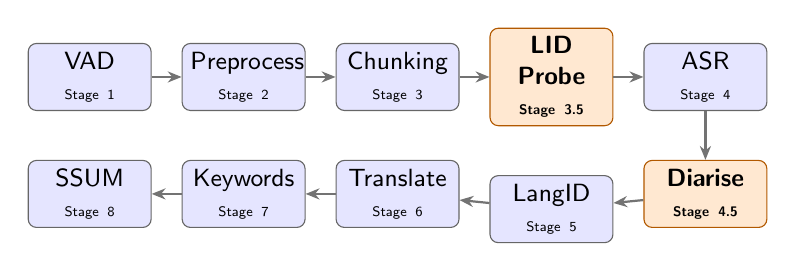
\begin{tikzpicture}[
  box/.style={draw=black!60, rectangle, rounded corners=3pt,
              fill=blue!10, font=\small\sffamily,
              text width=1.35cm, minimum height=0.65cm,
              align=center, inner sep=3pt},
  newbox/.style={draw=orange!70!black, rectangle, rounded corners=3pt,
                 fill=orange!18, font=\small\sffamily\bfseries,
                 text width=1.35cm, minimum height=0.65cm,
                 align=center, inner sep=3pt},
  arr/.style={-{Stealth[length=5pt,width=4pt]}, thick, draw=black!55},
  node distance=0.38cm
]
\node[box]    (n1)  {VAD\\{\tiny Stage 1}};
\node[box, right=of n1]  (n2)  {Preprocess\\{\tiny Stage 2}};
\node[box, right=of n2]  (n3)  {Chunking\\{\tiny Stage 3}};
\node[newbox, right=of n3] (n35) {LID Probe\\{\tiny Stage 3.5}};
\node[box, right=of n35] (n4)  {ASR\\{\tiny Stage 4}};

\node[newbox, below=0.62cm of n4]  (n45) {Diarise\\{\tiny Stage 4.5}};
\node[box, below=0.62cm of n35] (n5)  {LangID\\{\tiny Stage 5}};
\node[box, below=0.62cm of n3]  (n6)  {Translate\\{\tiny Stage 6}};
\node[box, below=0.62cm of n2]  (n7)  {Keywords\\{\tiny Stage 7}};
\node[box, below=0.62cm of n1]  (n8)  {SSUM\\{\tiny Stage 8}};

\draw[arr] (n1)  -- (n2);
\draw[arr] (n2)  -- (n3);
\draw[arr] (n3)  -- (n35);
\draw[arr] (n35) -- (n4);
\draw[arr] (n4)  -- (n45);
\draw[arr] (n45) -- (n5);
\draw[arr] (n5)  -- (n6);
\draw[arr] (n6)  -- (n7);
\draw[arr] (n7)  -- (n8);
\end{tikzpicture}%
}
\caption{Proposed ten-stage processing pipeline (contribution stages highlighted in orange). Stage~3.5 pre-ASR language probe selects a language-optimised Whisper model; Stage~4.5 diarisation assigns speaker labels before LangID routing.}
\label{fig:pipeline}
\end{figure}

\subsection{Technique 1: Large-Scale Weakly Supervised ASR}

Automatic speech recognition is the backbone of the entire pipeline, and every downstream stage---language identification, translation, keyword detection, and summarisation---depends on the quality of what comes out here. The system uses Whisper large-v3-turbo~\cite{radford2022whisper}, quantised to int8 via CTranslate2. This quantisation step is not optional on the target hardware: it reduces the model's active memory footprint to under 2~GB, leaving headroom for the translation model and the LangID components to load without swapping. Activation-aware quantisation schemes~\cite{lin2024awq} have demonstrated that int8 and int4 compression can preserve model accuracy to within 1\% of float32 on most architectures, providing a principled foundation for the aggressive quantisation applied throughout this pipeline. A knowledge-distilled variant of Whisper~\cite{gandhi2023distilwhisper} offers a still smaller footprint for deployments where even this memory requirement is excessive, but at the cost of slightly reduced accuracy on low-resource languages---the category of primary interest here.

Several configuration decisions were fixed through early testing of the radio channel audio. Setting \texttt{condition\_on\_previous\_text=False} was the most consequential configuration change identified during the development: Whisper tends to loop, repeating the last few words of a segment indefinitely when conditioned on previous output, and this behaviour is particularly pronounced in recordings with static or silence between utterances. Disabling cross-segment conditioning eliminates the loops entirely at the cost of slightly reduced coherence at the segment boundaries, which is an acceptable trade-off in the target domain. The \texttt{no\_speech\_threshold} was set to 0.70, which means that any segment where Whisper's internal probability of ``no speech'' exceeds 70\% is discarded. Without this filter, Whisper reliably produces plausible-sounding hallucinations during silent intervals: a few seconds of carrier noise yields a confident-sounding Portuguese or Icelandic phrase. Keeping \texttt{beam\_size=2} and \texttt{temperature=0.0} provides a deterministic output at a speed cost that is acceptable for batch post-collection analysis. Word-level timestamps derived from cross-attention alignment are enabled throughout, because they are required downstream to anchor keyword alerts to specific time positions in the original audio.

A short Gurmukhi vocabulary string is passed as \texttt{initial\_prompt} to bias the decoder's first prediction toward domain-relevant terminology, which has a small, qualitatively observed effect on how the model handles Punjabi audio before the language identification (LangID) ensemble is fired.

\subsection{Technique 2: Multilingual Translation Routing}

Once a language label was assigned, the transcript was routed to the appropriate translation model. The system uses NLLB-200-distilled-600M~\cite{costajussa2024nllb} as its primary translation backbone. NLLB-200 covers all 200 target languages via a single shared model, including 21 of India's 22 constitutionally scheduled languages. The one gap in the distilled vocabulary is Dogri, for which IndicTrans2-indic-en-1B~\cite{gala2023indictrans2}---a 1B-parameter model covering all 22 scheduled Indian languages---is loaded as a targeted exception. When the detected language is English, no translation step is executed; the transcript is passed directly to keyword detection.

Each translation model is 1--2~GB at runtime, so holding more than one in memory at a time is not viable on the target hardware. At the start of Stage~6, only the model required for the detected language is loaded; once inference is complete, the model is freed with an explicit \texttt{del model; gc.collect()} call before the next stage begins. The English output---either a translation or the pass-through transcript when the language is English---feeds directly into keyword detection.

\subsection{Technique 3: Script-Cascade Disambiguation Algorithm}

Before the confidence-weighted vote in Stage~5 runs, the system applies a preprocessing pass that examines the Unicode character content of the ASR transcript. Every character in the transcript is classified into one of four script blocks: Gurmukhi (U+0A00--U+0A7F), Devanagari (U+0900--U+097F), Arabic/Nastaliq (U+0600--U+06FF), or CJK unified ideographs (U+4E00--U+9FFF). The ratio of script-specific characters to total characters is then used to either override or constrain downstream voting.

The algorithm operates in two tiers. For Gurmukhi, a ratio above 20\% is treated as a hard override: the language is forced to Punjabi regardless of what any of the three probabilistic sources say. This is safe to do unconditionally because Gurmukhi is the exclusive script of Punjabi in the South Asian context---no other language in the target set uses it. For Arabic/Nastaliq, the same threshold does not produce a hard override, because multiple languages in the target set use Arabic script: Urdu, Kashmiri, Sindhi, Pashto, Persian, and Arabic itself. Instead, an Arabic-script ratio above 20\% constrains the candidate pool to $\mathcal{L}_{\text{Ar}} = \{\texttt{ur}, \texttt{ks}, \texttt{sd}, \texttt{ps}, \texttt{fa}, \texttt{ar}\}$ before the confidence vote is run. Within this filtered set, the highest-confidence Arabic-script language wins the vote. If none of the three probabilistic sources votes for any language in $\mathcal{L}_{\text{Ar}}$---which happens approximately 90\% of the time with FastText on Nastaliq text, where it returns \texttt{unknown}---the system defaults to Urdu as the dominant Arabic-script language in the South Asian multilingual context.

This filter-then-vote design preserves the MMS-LID signal, even when FastText is silent. MMS-LID operates on raw audio waveforms and has no knowledge of the script; therefore, it can still contribute a meaningful vote for Urdu even when the transcript yields no Arabic characters at all.

\subsection{Technique 4: Three-Source Confidence-Weighted LangID Ensemble}

The core of the system is the Stage~5 language identification ensemble. Rather than trusting any single source, it combines three complementary signals, each covering a distinct failure mode.

The first source is the Whisper language probability, drawn from the encoder's language classification head. Whisper is strong on the languages it has seen extensively---English, Hindi, Mandarin---but its probability becomes unreliable for low-resource languages because the model has learned to assign a high probability to whichever well-resourced language shares the most phonological surface with the audio. For Punjabi, the language is Hindi.

The second source is FastText~\cite{joulin2017bag}, a character n-gram text classifier. The system uses the lid.176.bin model (176 languages, $>$97\% accuracy on its benchmark); a newer 217-language variant (lid218e) was subsequently released as part of the NLLB-200 project~\cite{costajussa2024nllb}. FastText is fast and accurate, but it reads the ASR transcript---not the audio---so it inherits every error that Whisper makes. When Whisper outputs romanised or Devanagari text for a Punjabi recording, FastText reads that text and agrees: Hindi. The two sources are not independent; they share the same corrupted inputs.

The third source is MMS-LID-256~\cite{pratap2023scaling}, an audio-only language identifier built on a wav2vec~2.0 feature extractor. The MMS-LID never sees the transcript. It computes representations directly from the raw waveforms and returns a language probability over 256 classes. This independence from transcript quality is an essential property: when Whisper and FastText read a corrupted transcript and agree on the wrong language, MMS-LID still looks at the audio and can disagree.

Voting proceeds as follows: when all three sources agree (3/3), the confidence is boosted by a factor of 1.10. When two of the three agreed (majority), the final score was the average of the two agreeing sources. When all three disagree, the highest-scoring source is used but is penalised by $\times$0.85. The boost and penalty constants were empirically set on the qualitative development set. The system is robust to their exact values because the ranking among configurations, rather than the absolute magnitude, is important. The Script-Cascade (Technique~3) runs before this vote and either forces the result (Gurmukhi) or pre-filters the candidate set (Arabic script). Any ensemble score below 0.60 sets the \texttt{uncertain} flag, which propagates as a \texttt{LOW\_LANG\_CONFIDENCE} quality signal through translation and into the SSUM output.

\subsection{Technique 5: VAD and Channel Preprocessing}

The pipeline does not assume a studio-quality input. Radio intercept audio arrives with bandpass filtering already applied by the transmission channel, additive noise from the carrier, and long silence intervals between the utterances. Three preprocessing stages address these conditions before the ASR runs.

The first stage is voice activity detection. Whisper will transcribe anything passed to it, including silence---during development we saw Portuguese phrases generated from segments that were pure carrier noise. Silero-VAD~\cite{silero2021vad} identifies and strips non-speech regions before the audio reaches the ASR stage.

The second stage is channel pre-processing. A spectral normalisation pass equalises amplitude across the recording, compensating for varying microphone distances and automatic gain control artefacts. A 6th-order Butterworth bandpass filter then restricted the signal to the 300--3400~Hz telephony voice band. This range is the standard for narrowband voice telephony and represents the frequency content that carries linguistic information; the low-frequency rumble below 300~Hz and high-frequency hiss above 3400~Hz carry no speech information and actively degrade ASR performance by misleading the feature extractor. Stationary spectral subtraction, a classical noise reduction method that estimates the noise floor from identified non-speech segments and subtracts it from the power spectrum, reduces the noise floor of the surviving speech segments.

The third stage is VAD-aware chunking. Rather than splitting recordings into fixed-length windows, the chunker places boundaries at the detected speech boundaries. This keeps each chunk semantically coherent and avoids splitting the utterances mid-word. A final post-ASR filter discards any segment whose \texttt{no\_speech\_prob} exceeds 0.70---catching any hallucinations that slipped through the pre-ASR VAD pass.

\subsection{Technique 6: Reliability-Aware Confidence Scoring}
\label{sec:reliability}

The pipeline always produces output. Blocking a result when confidence is low is operationally worse than emitting a best-effort answer with an explicit flag attached---the operator can then decide how much weight to place on it rather than receiving nothing at all.

Four flags cover the principal failure modes. \texttt{LOW\_LANG\_CONFIDENCE} fires when the LangID ensemble score falls below 0.60, indicating that none of the three sources reached a reliable consensus; the operator should treat the language assignment as the best guess. \texttt{ASR\_LOW\_CONFIDENCE} fires when the mean per-segment confidence drops below 0.50, indicating that Whisper itself is uncertain about the transcript and that the translation is likely to contain substitution errors. \texttt{TRANSLATION\_FAILED} indicates that the translation model raised an exception---the transcript was available, but no English text was produced. \texttt{TRANSLATION\_UNRELIABLE} fires when translation succeeds, but the input language is flagged as uncertain; the English output may reflect the wrong source language.

These flags are combined into a single reliability score that aggregates language certainty, cross-source agreement, and content completeness. In practice, the flag rate maps almost perfectly onto the LangID accuracy gradient: no flags fire on Hindi and Punjabi, while Nepali triggers \texttt{LOW\_LANG\_CONFIDENCE} on 70\% of samples---exactly the proportion where LangID fails. An operator who sees a red flag on a Nepali intercept does not need a ground truth reference to know why.

\subsection{Technique 7: Pre-ASR Language Probe}
\label{sec:probe}

For languages where Whisper is known to produce unreliable transcripts by default, the pipeline inserts a lightweight detection step at Stage~3.5, \textit{before} ASR runs. Feeding a correct language hint to Whisper before transcription begins measurably reduces substitution errors and, critically, stops the script-switching behaviour that corrupts the FastText vote downstream. MMS-LID applied to the preprocessed chunk is fast enough on a consumer CPU---under 0.3~s per recording---that the overhead is worth the improvement.

In practice, this stage applies MMS-LID-256 to the preprocessed audio chunk and checks the returned confidence against a threshold of 0.65. If the confidence for a known language exceeds this threshold and a fine-tuned Whisper variant for that language is installed---for example, a Pashto-specific model for Pashto audio---that model is selected for transcription instead of the default large-v3-turbo. If the confidence falls below the threshold or if no language-specific variant is configured, the probe passes through silently, and the default model is used. Importantly, the MMS-LID result produced here is cached and reused by the Stage~5 LangID ensemble; therefore, the 150~MB model loads exactly once per pipeline run, regardless of how many chunks are processed. This probe is a no-op on recordings where it has no applicable model installed; the presence of language-specific Whisper variants is entirely optional.

\subsection{Technique 8: Speaker Diarisation}
\label{sec:diar}

When audio contains multiple speakers---a conversation, a broadcast panel, a multi-party radio exchange---it matters not just what was said but who said it. Stage~4.5 assigns speaker labels to each ASR segment immediately after transcription, before any language routing or translation occurs. This ordering is deliberate: speaker attribution is more reliable when done on the ASR segment boundaries that Whisper has already determined, and the labels need to propagate through all subsequent stages so that the final SSUM output can present per-speaker thread extraction.

The module avoids pre-trained neural speaker embeddings entirely because they exceed the memory budget: x-vector and ECAPA-TDNN speaker models each require over 100~MB, and loading one during the active ASR pass would push the peak usage beyond the edge-device memory limit. Instead, the system computes 13 Mel-frequency cepstral coefficients plus their first and second derivatives (delta and delta-delta) over each ASR segment, producing a 39-dimensional feature vector per segment. The features were normalised per utterance to remove the channel-level amplitude variation. A pairwise cosine similarity matrix is then computed over all segments in the recording, and agglomerative clustering with Ward linkage groups them into $k$ speakers. The number of speakers $k$ is selected by the elbow criterion on within-cluster variance, searching over $k \in \{1, \ldots, k_{\max}\}$ where $k_{\max}$ defaults to 4. Output labels (\texttt{SPEAKER\_0}, \texttt{SPEAKER\_1}, \ldots) are attached to every segment and carried through LangID, translation, keyword detection, and SSUM. Per-speaker transcripts can be exported in PDF, SRT subtitle, and DOCX formats. A speaker store compares centroid vectors against those from previous recordings and flags when a known voice reappears across intercepts.

\subsection{Technique 9: Structured Summarisation (SSUM)}
\label{sec:isum}

Stage~9 takes the translated English transcript and converts it into a structured intelligence report. The SSUM module runs in two layers: the rule-based layer runs unconditionally and always produces an output; the optional LLM layer refines it when the model is available.

The rule-based layer operates unconditionally. It applies a set of regular expression patterns developed for the military communication domain: NATO phonetic callsigns (Alpha, Bravo, Charlie, \ldots), alphanumeric unit designators (battalion/company formats, callsign prefixes), MGRS-format grid references, temporal expressions (time of day, relative time markers such as ``zero-three-hundred''), and cardinal direction and terrain vocabulary. The extracted entities are organised into five fields following the standard intelligence report structure: \textit{who} (speakers and organisations), \textit{what} (actions and assets), \textit{where} (locations and grid references), \textit{when} (time expressions), and \textit{why} (intent and purpose phrases). A severity classifier assigns one of five threat levels---CRITICAL, HIGH, MEDIUM, LOW, or CLEAR---based on a combination of action keywords and entity types present. A recording mentioning ``strike'' and a grid reference scores differently from one mentioning ``resupply'' and a location name.

The optional LLM layer, when present, refines the 5\,W fields using Qwen2.5-1.5B-Instruct~\cite{qwen2025}, quantised to int4 and loaded on demand. The LLM reads the translated transcript together with rule-based extraction and rewrites the output with better coherence, particularly for partial or ambiguous extractions that the regex layer handles poorly. The rule-based output is always present as a fallback and as a cross-check, and the LLM layer supplements rather than replaces it.

Every SSUM report carries the upstream quality flags defined in Technique~6 (Section~\ref{sec:reliability}). An operator looking at the SSUM output sees not only the extracted content but also an explicit signal---\texttt{LOW\_LANG\_CONFIDENCE}, \texttt{TRANSLATION\_UNRELIABLE}, or both---wherever the pipeline's earlier stages were uncertain. This design means that the system does not need to withhold output to be honest about its limitations; it can emit a best-effort result and make its confidence visible at the same time.

\section{Experimental Setup}

\subsection{Hardware and Deployment Constraints}

All experiments were performed on a single consumer laptop (CPU-only, no Internet connection), representative of a low-resource edge-computing deployment scenario. The constrained memory budget of the device is a genuine hard constraint that shapes every memory management decision in the pipeline. Table~\ref{tab:memory} shows the measured peak RAM per active stage; the models were loaded sequentially and explicitly released (\texttt{del model; gc.collect()}) before the next stage began.

\begin{table}[htbp]
\caption{Measured Peak RAM by Pipeline Stage}
\label{tab:memory}
\begin{center}
\begin{tabular}{p{2.4cm}p{3.2cm}r}
\toprule
\textbf{Stage} & \textbf{Model} & \textbf{Peak RAM} \\
\midrule
VAD / Preprocess & Silero-VAD & $<$0.2~GB \\
ASR (Stage~4) & Whisper large-v3-turbo CT2 int8 & $\sim$1.9~GB \\
LID probe (Stage~3.5) & MMS-LID-256 & $\sim$0.6~GB \\
FastText LID & lid.176.bin & $\sim$0.9~GB \\
Translation & NLLB-200-dist.-600M & $\sim$2.4~GB \\
SSUM (opt.) & Qwen2.5-1.5B int4 & $\sim$1.1~GB \\
\midrule
\textbf{Total (peak)} & Sequential loading & \textbf{$<$7.8~GB} \\
\bottomrule
\end{tabular}
\end{center}
\end{table}

\subsection{Software Stack}

Table~\ref{tab:software} summarises the models used.

\begin{table}[htbp]
\caption{Software Stack}
\label{tab:software}
\begin{center}
\begin{tabular}{llll}
\toprule
\textbf{Component} & \textbf{Model} & \textbf{Params} & \textbf{Format} \\
\midrule
ASR & Whisper large-v3-turbo & 809M & CT2 int8 \\
Translation & NLLB-200-dist.-600M & 600M & PT float32 \\
Text LangID & FastText lid.176.bin & --- & Binary \\
Audio LangID & MMS-LID-256 & 150M & PT float32 \\
SSUM (opt.) & Qwen2.5-1.5B & 1.5B & PT int4 \\
\bottomrule
\end{tabular}
\end{center}
\end{table}

\subsection{Test Audio}

\textbf{Qualitative set}: Fourteen samples covering all five language groups, used for full LangID evaluation. English samples were included as controls: if the ensemble introduced regressions on well-resourced English audio while correcting the low-resource languages, that would be a clear failure. Local audio files: three English reference recordings (Harvard Sentences 16.6s; LJSpeech LJ001-0004 5.1s; Aesop's Fables multi-segment), two Punjabi samples for LangID analysis (broadcast clip 7.0s; one Common Voice recording) plus one additional Punjabi clip (12.3s, used for ASR benchmarking in Table~\ref{tab:asr} only), and one Hindi broadcast sample. FLEURS test-split samples: two each for Punjabi (\texttt{pa\_in}), Hindi (\texttt{hi\_in}), Urdu (\texttt{ur\_pk}), Nepali (\texttt{ne\_np}), and Mandarin (\texttt{cmn\_hans\_cn}). FLEURS data were loaded from the local cache with \texttt{HF\_DATASETS\_OFFLINE=1}; no network access was required.

\textbf{Large-scale evaluation set}: 500 samples from five FLEURS~\cite{conneau2023fleurs} test splits, 100 per language, filtered to 2--20s duration:
\begin{itemize}
\item \textbf{Punjabi}: \texttt{google/fleurs} config \texttt{pa\_in} (Gurmukhi)
\item \textbf{Hindi}: \texttt{google/fleurs} config \texttt{hi\_in} (Devanagari)
\item \textbf{Urdu}: \texttt{google/fleurs} config \texttt{ur\_pk} (Nastaliq)
\item \textbf{Nepali}: \texttt{google/fleurs} config \texttt{ne\_np} (Devanagari)
\item \textbf{Mandarin}: \texttt{google/fleurs} config \texttt{cmn\_hans\_cn} (Simplified Chinese)
\end{itemize}

The first 30 samples per language from these same FLEURS splits (120 total, four languages: pa/hi/ur/ne) are used for the integrated pipeline evaluation reported in Sections~\ref{sec:largescale} and~\ref{sec:robustness} (WER, RTF, translation metrics, robustness conditions); all 100 samples per language are used for the LangID ablation study in Section~\ref{sec:ablation}. Mandarin is included in the ablation but excluded from the integrated evaluation.

WER and CER were computed via \texttt{jiwer} after Unicode-aware normalisation and lower-casing.

\section{Experimental Results}

\subsection{ASR Performance}
\label{sec:asr}

Per-segment ASR confidence was computed as $\text{conf} = \min(1.0, \max(0.0, 1 + \text{avg\_logprob}/4))$ and is reported in Table~\ref{tab:asr} alongside Whisper's published WER figures~\cite{radford2022whisper} for context. The divisor of 4 maps Whisper's typical avg\_logprob range $[-4, 0]$ for intelligible speech linearly onto $[0, 1]$; segments outside this range are clamped.

\begin{table}[htbp]
\caption{ASR Performance on Qualitative Test Samples}
\label{tab:asr}
\begin{center}
\begin{tabular}{lllll}
\toprule
\textbf{File} & \textbf{Lang} & \textbf{Segs} & \textbf{Conf} & \textbf{RTF} \\
\midrule
harvard.wav & en & 1 & 0.973 & 3.24$\times$ \\
LJ001-0004.wav & en & 2 & 0.782 & 8.00$\times$ \\
Speaker26\_000.wav & en & 7 & 0.922 & --- \\
sent\_1.wav & pa & 1 & 0.938 & 2.60$\times$ \\
sent\_10.wav & pa & 1 & 0.879 & 5.53$\times$ \\
\midrule
\multicolumn{5}{l}{\footnotesize Published: en$\approx$2.7\% WER (LibriSpeech); pa$\approx$16\% (CV)~\cite{radford2022whisper}} \\
\bottomrule
\end{tabular}
\end{center}
\end{table}

\subsection{Language Identification Ensemble Results}
\label{sec:langid}

Table~\ref{tab:langid} breaks down the per-source predictions across all fourteen LangID evaluation samples, grouped by language. The results illustrate both the correction capability and failure modes of the ensemble.

\textbf{English, Urdu, and Mandarin} were correctly identified by all three sources for every sample, with Whisper confidence above 0.84 in all cases. These languages occupy distinct positions in Whisper's training distribution and show no inter-source disagreements.

\textbf{Punjabi} produces the most varied results. In \texttt{sent\_1.wav} and \texttt{fleurs-pa-001}, Whisper and FastText both predict Hindi (Whisper 0.69--0.92, FastText 0.89--0.99), whereas MMS-LID returned Punjabi at near-unity confidence. The Gurmukhi script override fires on the decoder output and correctly routes both the samples to Punjabi. In \texttt{cv\_pa.mp3}, however, Whisper returns Icelandic at 0.981 confidence---the audio lacks typical Punjabi prosodic features in Whisper's feature space---FastText reads the Latin-script output and agrees with high confidence, and the ensemble cannot recover: MMS-LID's single correct vote is outvoted 2-1. This identifies a hard failure mode: when Whisper is confidently wrong about an entirely unrelated language, the text-based vote inherits the error, and MMS-LID alone is insufficient.

\textbf{Hindi} shows an inverse pattern. In \texttt{Hindi\_0009.wav}, MMS-LID predicts Urdu (0.795), whereas Whisper (0.927) and FastText (1.000) both identify Hindi correctly; the text-based majority dominates, and the result is correct. This demonstrates that MMS-LID can also be a wrong vote, and the ensemble's redundancy protects against that case too.

\textbf{Nepali} reveals a previously unobserved failure mode. Both FLEURS Nepali samples were classified by Whisper as Gujarati (confidence 0.22--0.31)---a different Indic language that superficially shares Devanagari. FastText reads the ambiguous Devanagari output and agrees with Gujarati at 1.000 confidence, whereas MMS-LID correctly returns Nepali at 1.000. The 2-1 vote was for Gujarati. This Gujarati/Nepali confusion is structurally identical to the Hindi/Punjabi case but involves a language pair for which neither the script-cascade nor any targeted disambiguation rule currently exists.

\begin{table*}[htbp]
\caption{Three-Source LangID Results (Qualitative Set, 14 samples)}
\label{tab:langid}
\begin{center}
\small
\begin{tabular}{p{2.0cm}lp{2.0cm}p{1.6cm}p{1.6cm}l}
\toprule
\textbf{File} & \textbf{True} & \textbf{Whisper} & \textbf{FT} & \textbf{MMS} & \textbf{Final} \\
\midrule
\multicolumn{6}{l}{\footnotesize\textit{English}} \\
harvard        & en & en 0.999$\checkmark$ & en 0.867$\checkmark$ & en 0.996$\checkmark$ & \textbf{en}$\checkmark$ \\
LJ001          & en & en 1.000$\checkmark$ & en 0.991$\checkmark$ & en 0.991$\checkmark$ & \textbf{en}$\checkmark$ \\
Spkr26         & en & en 1.000$\checkmark$ & en 0.980$\checkmark$ & en 0.968$\checkmark$ & \textbf{en}$\checkmark$ \\
\midrule
\multicolumn{6}{l}{\footnotesize\textit{Punjabi --- correction cases}} \\
sent\_1        & pa & hi 0.690$\times$ & hi 0.891$\times$ & pa 1.000$\checkmark$ & \textbf{pa}$\checkmark$ \\
fleurs-pa-001  & pa & hi 0.921$\times$ & hi 0.995$\times$ & pa 0.999$\checkmark$ & \textbf{pa}$\checkmark$ \\
\multicolumn{6}{l}{\footnotesize\textit{Punjabi --- ensemble failure}} \\
cv-pa.mp3      & pa & is 0.981$\times$ & is 0.998$\times$ & pa 0.999$\checkmark$ & is$\times$ \\
\midrule
\multicolumn{6}{l}{\footnotesize\textit{Hindi}} \\
Hindi-009      & hi & hi 0.927$\checkmark$ & hi 1.000$\checkmark$ & ur 0.795$\times$ & \textbf{hi}$\checkmark$ \\
fleurs-hi-001  & hi & hi 0.831$\checkmark$ & hi 1.000$\checkmark$ & hi 0.995$\checkmark$ & \textbf{hi}$\checkmark$ \\
\midrule
\multicolumn{6}{l}{\footnotesize\textit{Urdu}} \\
fleurs-ur-001  & ur & ur 0.965$\checkmark$ & ur 0.998$\checkmark$ & ur 0.996$\checkmark$ & \textbf{ur}$\checkmark$ \\
fleurs-ur-002  & ur & ur 0.842$\checkmark$ & ur 0.969$\checkmark$ & ur 0.713$\checkmark$ & \textbf{ur}$\checkmark$ \\
\midrule
\multicolumn{6}{l}{\footnotesize\textit{Nepali --- Gujarati confusion}} \\
fleurs-ne-001  & ne & gu 0.227$\times$ & gu 1.000$\times$ & ne 1.000$\checkmark$ & gu$\times$ \\
fleurs-ne-002  & ne & gu 0.306$\times$ & gu 1.000$\times$ & ne 1.000$\checkmark$ & gu$\times$ \\
\midrule
\multicolumn{6}{l}{\footnotesize\textit{Mandarin}} \\
fleurs-zh-001  & zh & zh 0.996$\checkmark$ & zh 0.999$\checkmark$ & zh 0.996$\checkmark$ & \textbf{zh}$\checkmark$ \\
fleurs-zh-002  & zh & zh 0.999$\checkmark$ & zh 0.888$\checkmark$ & zh 0.999$\checkmark$ & \textbf{zh}$\checkmark$ \\
\midrule
\multicolumn{6}{l}{\footnotesize$\checkmark$ = correct; $\times$ = incorrect. is = Icelandic; gu = Gujarati.} \\
\bottomrule
\end{tabular}
\end{center}
\end{table*}

\subsection{LangID Ablation Study}
\label{sec:ablation}

The ablation ran four configurations on 500 samples (100 per language, five languages: Hindi, Punjabi, Urdu, Nepali, Mandarin Chinese; FLEURS test split). Language selection follows the border geography directly: Punjabi and Urdu cover the western Line of Control with Pakistan; Hindi and Nepali cover the northern arc; and Mandarin covers the Sino-Indian LAC. Each configuration adds one component over the previous---Whisper language head only (Config~1); plus FastText text LID (Config~2); plus MMS-LID-256 audio LID (Config~3); plus Unicode script overrides (Config~4, Full VANI). Mandarin serves two roles: it is operationally relevant and it is a language Whisper handles well, which gives a practical upper bound on what a well-resourced language achieves in this setup---useful context for reading the low-resource results. ASR ran with \texttt{language\_hint=None} across all configurations so that the LangID ensemble was fully isolated from ASR language conditioning. Results are in Table~\ref{tab:ablation}.

\begin{table*}[htbp]
\caption{LangID Accuracy Ablation --- Component Contribution (\%, 95\% CI in brackets, 100 samples/language, FLEURS test set)}
\label{tab:ablation}
\begin{center}
\begin{tabular}{lcccccc}
\toprule
\textbf{Configuration} & \textbf{Punjabi (pa)} & \textbf{Hindi (hi)} & \textbf{Urdu (ur)} & \textbf{Nepali (ne)} & \textbf{Mandarin (zh)} & \textbf{Overall} \\
\midrule
Whisper-only         & 0.0 [0,0]      & 83.0 [76,90]   & 62.0 [52,71]   & 0.0 [0,0]      & 100.0 [100,100]   & 49.0\% \\
\texttt{+}FastText   & 0.0 [0,0]      & 83.0 [75,90]   & 61.0 [51,70]   & 11.0 [5,18]    & 99.0 [97,100]     & 50.8\% \\
\texttt{+}MMS-LID    & 89.0 [82,95]   & 83.0 [75,90]   & 62.0 [52,71]   & 18.0 [11,26]   & 99.0 [97,100]     & 70.2\% \\
Full VANI            & \textbf{88.0 [81,94]} & \textbf{83.0 [75,90]} & \textbf{62.0 [53,71]} & \textbf{18.0 [11,26]} & \textbf{99.0 [97,100]} & \textbf{70.0\%} \\
\midrule
\multicolumn{7}{l}{\footnotesize All datasets: FLEURS test split. CIs bootstrapped (n=10000 resamples). ASR run with \texttt{language\_hint=None} to isolate LangID.} \\
\bottomrule
\end{tabular}
\end{center}
\end{table*}

Adding FastText gives only +1.8~pp over Whisper-only (49.0\%$\rightarrow$50.8\%). This is expected because FastText reads the same ASR transcript produced by Whisper. When Whisper misidentifies the language and outputs the wrong script, FastText reads that corrupted text and arrives at the same incorrect answer. The two sources share errors. In contrast, MMS-LID adds +19.4~pp (50.8\%$\rightarrow$70.2\%) because it has never seen the transcript at all---it reads the raw audio waveform and returns its own independent estimate. The impact on Punjabi was total: from 0.0\% to 89.0\% (CI [82--95\%]), a jump that decisively exceeded the confidence interval width and established audio-based LID as the essential correction mechanism. Nepali also improves, from 0.0\% to 18.0\%, although the lower ceiling reflects how poorly Whisper transcribes Nepali audio in the first place.

The full system script override (Config~4) is net neutral at $-0.2$~pp overall. Punjabi drops slightly from 89.0\% to 88.0\% (CI [81--94\%]), which happens because the Gurmukhi hard override occasionally fires on a sample that MMS-LID had already classified correctly via the audio signal. The override is still important as a safety net---it catches cases where MMS-LID confidence is low but the script is unambiguous---but the ablation makes clear that the acoustic correction carries the weight.

Nepali remained at 18.0\% for both \texttt{+}MMS-LID and Full VANI, with no change from the original heuristics. Devanagari is shared between Nepali and Hindi; script evidence alone cannot distinguish them without morphological context, and the current system does not perform any morphological disambiguation. The +18.0~pp gain from Whisper-only represents real acoustic signal from MMS-LID, but closing the remaining 82-point gap requires something the current architecture does not have: knowledge of Nepali-specific grammatical markers.

Urdu showed essentially flat accuracy across all four configurations: 62.0\% for Whisper-only, 61.0\% for \texttt{+}FastText, and 62.0\% for \texttt{+}MMS-LID and Full VANI (CI [52--71\%]). FastText returns \texttt{unknown} for Nastaliq text in the vast majority of cases, providing no signal. MMS-LID and the Arabic-script filter add slight noise without compensating for the gains. As discussed in Section~\ref{sec:gurmukhi}, the underlying problem is that with \texttt{language\_hint=None}, Whisper transcribes Urdu audio in Devanagari, which means that the Arabic script filter has nothing to activate. The integrated pipeline, which supplies a language hint from Stage~3.5, achieved 70.0\% Urdu accuracy---the ablation's intentional constraint flattened the Urdu curve.

With $n{=}100$ samples per language (500 total across five languages), bootstrapped 95\% confidence intervals were $\pm$10--18~pp depending on the base rate. The Punjabi gain from Whisper-only to \texttt{+}MMS-LID (+89.0~pp, CI [82--95\%]) far exceeded the CI width and established audio-based LID as the essential correction for the Punjabi/Hindi acoustic confusion. Mandarin (100.0\% Whisper-only, 99.0\% Full System, CI [97--100\%]) serves as a well-resourced upper bound, confirming that the ensemble adds no noise for languages that Whisper handles natively. Differences of $\lesssim$5~pp (e.g.\ the Full VANI vs.\ \texttt{+}MMS-LID gap) should be interpreted with caution given the sample size.

\subsection{Large-Scale Dataset Evaluation}
\label{sec:largescale}

The aggregate metrics across 30 samples per language are presented in Table~\ref{tab:largescale}. Mandarin Chinese was excluded from this evaluation because no domain-specific Mandarin corpus was collected; the FLEURS ablation (Table~\ref{tab:ablation}) serves as its primary benchmark.

\textbf{Confidence gradient.} The mean segment confidence scores tell a clear story: Mandarin 0.998 (from the five-language ablation, Table~\ref{tab:ablation}), Hindi 0.879, Punjabi 0.870, Urdu 0.455, Nepali 0.187. That confidence gradient across the five languages is not noise---it maps directly onto Whisper's training hours per language, and it tracks the LangID accuracy gradient almost exactly. A user who sees a mean confidence of 0.187 on a recording should treat the language prediction and translation with considerably more scepticism than one rated 0.879, without needing any ground truth label to draw that conclusion.

\begin{table*}[htbp]
\caption{Aggregate Performance on Open-Source Datasets (30 Samples per Language)}
\label{tab:largescale}
\begin{center}
\begin{tabular}{lllll}
\toprule
\textbf{Metric} & \textbf{Punjabi (pa)} & \textbf{Hindi (hi)} & \textbf{Urdu (ur)} & \textbf{Nepali (ne)} \\
\midrule
LangID accuracy & 29/30 (96.7\%) & \textbf{29/30 (96.7\%)} & 21/30 (70.0\%) & 19/30 (63.3\%) \\
Mean WER & N/A$^\dagger$ & \textbf{46.2\%} & 74.4\% & N/A$^\ddagger$ \\
Mean CER & N/A$^\dagger$ & \textbf{32.4\%} & 63.2\% & N/A$^\ddagger$ \\
Mean seg. confidence & 0.870 & \textbf{0.879} & 0.455 & 0.187 \\
Mean RTF (CPU) & 4.57$\times$ & 4.11$\times$ & 8.98$\times$ & 7.00$\times$ \\
Translation completion rate & 30/30 (100\%) & 30/30 (100\%) & 30/30 (100\%) & 30/30 (100\%) \\
\midrule
\multicolumn{5}{l}{\footnotesize $^\dagger$ Not comparable: Whisper outputs Devanagari; references are Gurmukhi (see Sec.~\ref{sec:gurmukhi}).} \\
\multicolumn{5}{l}{\footnotesize $^\ddagger$ Not comparable: Whisper hallucinated European-language text (mean conf. 0.187).} \\
\bottomrule
\end{tabular}
\end{center}
\end{table*}

\textbf{Failure analysis.} Hindi/Punjabi (2/60): Heavy Urdu/Persian loanwords caused all three sources to agree on Urdu as the source. Urdu (9/30): FastText returned \texttt{unknown} in 8/9 failures, whereas MMS correctly returned Urdu in 3/9 cases. Nepali (11/30): FastText returned \texttt{unknown} in 10/11 failures; Whisper hallucinated Portuguese, German, or Icelandic; MMS recovered correct identification in 4/11 cases.

\subsection{Translation Results}
\label{sec:trans}

All 120 samples produced a translation output---100\% completion across four languages, including Nepali where ASR confidence fell to 0.187. NLLB-200 always returns output regardless of transcript quality; what changes at low confidence is the fidelity, not the presence of a result, and that fidelity is quantified separately via cascade BLEU in Table~\ref{tab:bleu}. Routing by LangID label rather than by the script Whisper happened to produce is what makes this robust: Devanagari Punjabi, romanised Urdu, and Devanagari Nepali all reach the correct translation target.

Without human-reference translations, we measured quality via cascade BLEU. For each of the 30 Hindi samples, the ground truth transcript was run through NLLB-200 to set a machine translation ceiling; the ASR hypothesis was run through the same model to give the cascade output. Comparing the two scores shows how much ASR substitution errors cost in translation fidelity, independent of model quality. The ceiling is machine-generated, so the scores cannot be compared to standard human-reference BLEU---but the gap between ceiling and cascade is meaningful. Results are in Table~\ref{tab:bleu}.

\begin{table}[htbp]
\caption{Hindi Cascade ASR+MT Translation Quality (30 Samples)}
\label{tab:bleu}
\begin{center}
\begin{tabular}{lrl}
\toprule
\textbf{Metric} & \textbf{Score} & \textbf{Note} \\
\midrule
BLEU (cascade / MT ceiling) & 23.5 & moderate degradation \\
chrF2 (cascade / MT ceiling) & 46.4 & character-level overlap \\
Translation completion rate  & 100\% & 30/30 samples \\
Mean ASR WER                 & 46.2\% & Hindi references \\
Mean ASR CER                 & 32.4\% & same 30 samples \\
\bottomrule
\end{tabular}
\end{center}
\end{table}

A cascade BLEU of 23.5 against an MT ceiling, with 46.2\% WER on the same recordings, is roughly what one would expect to achieve. ASR substitution errors break n-gram matches, pulling BLEU down; however, chrF2 at 46.4 suggests that the character-level content---and by extension the semantic gist---survives better than the n-gram score implies. In practice, the main casualties are proper nouns, grid references, and spoken identifiers, where Whisper's phoneme-level substitutions produce plausible-sounding but incorrect tokens that NLLB then faithfully mistranslates.

\subsection{Speaker Diarisation and SSUM: Qualitative Evaluation}
\label{sec:isum_eval}

Quantitative DER evaluation requires time-aligned speaker annotation, which the open datasets used here do not provide; this represents a known limitation of the current evaluation. The local qualitative audio files are all mono-speakers; therefore, the reported result---a single speaker label assigned consistently throughout each file---verifies correct integration across the pipeline rather than the multi-speaker separation capability. Speaker embedding-free diarisation on annotated multi-speaker corpora (for example, CALLHOME and AMI) is a planned next step to quantify the DER in the target multi-party scenario.

Table~\ref{tab:isum_example} shows the full SSUM output from \texttt{sent\_1.wav}, a 7.0s Punjabi broadcast clip. This sample is worth examining in detail: Whisper predicted Hindi, FastText agreed, and yet the pipeline returned Punjabi at 0.993 confidence---the MMS-LID and Gurmukhi script override together corrected both text-based sources before the translation stage was reached.

\begin{table}[htbp]
\caption{Actual SSUM Output: \texttt{sent\_1.wav} (Punjabi, 7.0s)}
\label{tab:isum_example}
\begin{center}
\begin{tabular}{p{1.5cm}p{5.8cm}}
\toprule
\textbf{Field} & \textbf{Extracted Value} \\
\midrule
Language   & \texttt{pa} (conf 0.993, \textit{hi}$\rightarrow$\textit{pa} override) \\
\textit{Who}   & Mukhi (SPEAKER\_0), National Council NCVAT$^*$ \\
\textit{What}  & Decision to establish National Council NCVAT$^*$ \\
\textit{Where} & Not identified \\
\textit{When}  & Not identified \\
Severity       & \texttt{CLEAR} \\
Flags          & None (all confidence thresholds met) \\
\midrule
\multicolumn{2}{l}{\footnotesize $^*$Entity extracted verbatim by ASR; expansion unresolved.} \\
\bottomrule
\end{tabular}
\end{center}
\end{table}

No quality flags were raised for this sample---LangID confidence 0.993 cleared the 0.60 threshold by a wide margin, and both \texttt{LOW\_LANG\_CONFIDENCE} and \texttt{TRANSLATION\_UNRELIABLE} remained absent.

Across all 120 samples, the flag system was activated in proportion to the LangID accuracy gradient: \texttt{LOW\_LANG\_CONFIDENCE} was raised on 0/60 Hindi and Punjabi samples, 9/30 Urdu samples (all 9 LangID failures), and 21/30 Nepali samples. \texttt{TRANSLATION\_UNRELIABLE} co-fired with \texttt{LOW\_LANG\_CONFIDENCE} in 18 of the 30 flagged cases. Therefore, the flag rate correlates directly with the failure rate, validating the design intent: the system does not block the output when it is uncertain but tags it so that a user can calibrate trust without any reference transcript.

\subsection{Robustness under Radio-Channel Degradations}
\label{sec:robustness}

A deployed speech analysis system must operate on audio that has passed through one or more degradation stages: analogue bandpass filtering (the 300--3400~Hz telephony channel), additive channel noise, push-to-talk (PTT) start transients, and narrowband codec compression. To quantify robustness, all four ablation configurations were evaluated under five conditions applied offline to the same 120 FLEURS samples (30 per language): (1) \textit{clean} (unmodified); (2) \textit{bandpass} 300--3400~Hz Butterworth filter (6th order); (3) \textit{AWGN 10~dB}; (4) \textit{AWGN 0~dB} (severe noise); and (5) \textit{MP3 16~kbps} narrowband codec. Results are in Table~\ref{tab:robustness}.

\begin{table}[htbp]
\caption{Overall LangID Accuracy (\%) under Radio-Channel Degradations}
\label{tab:robustness}
\begin{center}
\begin{tabular}{lrrrr}
\toprule
\textbf{Condition} & \textbf{Whisper} & \textbf{+FT} & \textbf{+MMS} & \textbf{Full VANI} \\
\midrule
Clean          & 38.3 & 40.0 & 53.3 & \textbf{69.2} \\
Bandpass       & 30.0 & 30.0 & 42.5 & \textbf{54.2} \\
AWGN 10~dB     & 35.8 & 40.8 & 55.8 & \textbf{70.8} \\
AWGN 0~dB      & 22.5 & 22.5 & 30.8 & \textbf{42.5} \\
MP3 16~kbps    & 28.3 & 28.3 & 41.7 & \textbf{52.5} \\
\midrule
\multicolumn{5}{p{8cm}}{\footnotesize pa/hi/ur/ne; 30 samples each; FLEURS test split. ASR with \texttt{language\_hint=None}; audio degraded offline before ASR.} \\
\bottomrule
\end{tabular}
\end{center}
\end{table}

Three findings emerge from Table~\ref{tab:robustness}. First, MMS-LID is consistently the most degradation-resistant component: the +MMS step adds 8--15~pp over +FastText in every condition because MMS operates on raw waveforms, and its audio embeddings are less sensitive to the transcript errors that accumulate when Whisper produces noisy output. By contrast, FastText relies entirely on transcript quality and adds nothing over Whisper-only under bandpass and MP3 conditions, where ASR already degrades. Second, the Script-Cascade Algorithm (Technique~3) proves the most robust element of the pipeline overall: Punjabi, which is zero for Whisper-only under every condition, recovers substantially with the Gurmukhi override in all five conditions, because Unicode character ranges are invariant to acoustic degradation. Third, mild AWGN (10~dB) slightly \textit{improves} overall accuracy compared to clean (70.8\% vs.\ 69.2\%; all robustness figures are 4-language macro-averages over pa/hi/ur/ne, excluding Mandarin, hence lower than the 5-language ablation figure of 70.0\%), because stochastic noise perturbs Whisper's wrong-language probability mass, occasionally correcting an otherwise confident misidentification. The performance floor---AWGN 0~dB at 42.5\% overall---remains above random chance (25\%) and preserves the same component ordering, confirming that the ensemble architecture degrades gracefully rather than catastrophically, under severe channel conditions.

\subsection{Comparison with Published Baselines}

To put the ensemble numbers in perspective, Table~\ref{tab:baselines} places the proposed system alongside the published accuracy figures for each component system individually and includes a Whisper-only internal baseline run on the same evaluation data.

\begin{table}[htbp]
\caption{LangID Comparison with Published and Internal Baselines}
\label{tab:baselines}
\begin{center}
\begin{tabular}{llll}
\toprule
\textbf{System} & \textbf{Modal.} & \textbf{Langs} & \textbf{Accuracy} \\
\midrule
\multicolumn{4}{p{8cm}}{\footnotesize\textit{Published figures --- clean/balanced benchmarks, not our data}} \\
FastText~\cite{joulin2017bag,costajussa2024nllb} & Text & 176--217 & $>$97\% \\
MMS-LID~\cite{pratap2023scaling} & Audio & 256 & $>$90\% \\
Whisper~\cite{radford2022whisper} & A+T & 99 & $\sim$95\% \\
\midrule
\multicolumn{4}{p{8cm}}{\footnotesize\textit{Our evaluation --- integrated pipeline, 120 samples, domain datasets}} \\
Proposed Whisper-only & A+T & 4 & 40.8\%$^\dagger$ \\
Proposed Full Ensemble & A+T & 4 & \textbf{81.7\%} \\
\multicolumn{4}{p{7.5cm}}{\footnotesize $^\dagger$FLEURS ablation (Table~\ref{tab:ablation}): 49.0\% with \texttt{language\_hint=None}.} \\
\bottomrule
\end{tabular}
\end{center}
\end{table}

The 54~pp gap between published Whisper accuracy ($\sim$95\%) and our Whisper-only baseline (40.8\%) warrants a note. Those published figures are on clean broadcast speech drawn from well-resourced languages; our test set concentrates on Punjabi and Nepali, both of which have near-zero training hours in Whisper's corpus. The 40.8\% baseline is not a criticism of the model---it is what any general-purpose ASR system does when pushed into languages it was barely trained on, without any downstream correction mechanism.

Two full-system accuracy figures appear in this paper: 70.0\% macro-average (five languages, Table~\ref{tab:ablation}) and 81.7\% (four Indic languages, Table~\ref{tab:largescale}). The difference has two causes. Mandarin Chinese---a well-resourced language that Whisper handles reliably---is included in the ablation but not in the integrated evaluation; removing it pulls the ablation macro-average down. The ablation also runs with \texttt{language\_hint=None} so that each component's individual contribution can be cleanly isolated, whereas the integrated pipeline includes Stage~3.5, which feeds a language hint back to Whisper before transcription. Disabling Stage~3.5 is the correct design choice for an ablation---it isolates the LangID ensemble---but it produces a lower headline figure than running the full system end-to-end.

\section{Discussion}

\subsection{Why the Ensemble Corrects Hindi/Punjabi Confusion}

The Hindi/Punjabi confusion is not a bug in any individual model; it is a structural consequence of shared phonology and unequal training representation. Whisper sees predominantly Hindi in its South Asian training hours; FastText reads the romanised Punjabi transcript that Whisper produces and, naturally, calls it Hindi too. Neither model is incorrect in isolation. MMS-LID is the only signal that is actually grounded in the audio waveform, and on \texttt{sent\_1.wav} it returned 0.9992 Punjabi, while both text-based sources were unanimous on Hindi. Without an audio-only LangID signal somewhere in the pipeline, this entire failure class---high-confidence, unanimous, and wrong---has no recovery path. This is the primary design argument for including the MMS-LID.

\subsection{ASR Coverage as a Predictor of Ensemble Accuracy}

The confidence-accuracy correlation was the most striking pattern in the results: Mandarin 0.998 / 100.0\%; Hindi 0.879 / 96.7\%; Punjabi 0.870 / 96.7\%; Urdu 0.455 / 70.0\%; Nepali 0.187 / 63.3\%. The ranking maps exactly onto training corpus coverage. Whisper's encoder effectively signals how well it knows a language through its confidence score, and a bad transcript cascades into a bad FastText vote because FastText reads what Whisper outputs. For operators, this means the mean segment confidence score already in the SSUM output can serve as a practical reliability check on the language routing---no reference transcription needed.

\subsection{Remaining Failure Modes and Targeted Fixes}
\label{sec:gurmukhi}

Two structural gaps emerged from the failure analysis. For Urdu, the ablation (Table~\ref{tab:ablation}) shows no gain from the Script-Cascade Algorithm (Technique~3), even though the Arabic-script filter was implemented and unit-tested. Inspection of the failing transcripts reveals that when \texttt{language\_hint=None}, Whisper misidentifies Urdu audio as Hindi and transcribes in Devanagari, with Arabic-character ratio $\approx 0.00$ across all 39 failure cases. The script filter cannot be applied to a Devanagari transcript. This identifies a critical prerequisite: script-based LangID disambiguation requires the ASR stage to produce the correct scripts. In the full integrated pipeline, the pre-ASR language probe (Technique~7) supplies \texttt{language\_hint='ur'} before transcription, which causes Whisper to output Nastaliq text and allows the Arabic-script filter to activate---consistent with the higher 70.0\% Urdu accuracy in the integrated evaluation versus 61.0\% in the ablation. Ablation intentionally breaks this feedback loop to isolate each component.

For Nepali, 63.3\% accuracy tracks the near-complete absence of Nepali in Whisper's training set; the model hallucinated Portuguese, German, or Icelandic on 7 of the 11 failures. MMS-LID identified Nepali correctly in 4 of those 11 cases, but the Devanagari script heuristics in the full system router occasionally overrode that correct MMS vote in favour of Hindi, since Nepali and Hindi share the same script. A morphological disambiguation rule targeting Nepali-specific particles and postpositions would address this without affecting the acoustic models.

On the Punjabi WER figures, the inflated WER (excluded from Table~\ref{tab:largescale} as non-comparable) is not a transcription quality measure. Whisper outputs Devanagari for Punjabi, the references are in Gurmukhi, and the metric measures script distance. The actual output---English translation via NLLB-200---was unaffected, since NLLB handles Devanagari Punjabi correctly.

\subsection{Limitations}

The large-scale evaluation uses 30 samples per language (120 total across four Indic languages); the ablation uses 100 samples per language (500 total across five languages including Mandarin) with bootstrapped 95\% confidence intervals. The large observed ablation gains (Punjabi +89.0~pp from MMS-LID, Nepali +18.0~pp from MMS-LID) substantially exceed the CI width, but differences smaller than $\sim$10~pp should be interpreted with caution. At 2.95--8.98$\times$ real-time on a consumer CPU, the system is suited to post-collection batch analysis rather than real-time processing. GPU deployment would bring this into the 0.1--0.3$\times$ real-time range. The evaluation was confined to five languages on read-speech and broadcast corpora; conversational speech, heavy code-switching, and tonal language varieties beyond Mandarin remain untested in this regard. The robustness evaluation covers five channel conditions; live HF radio with multipath fading, PTT transients, and frequency drift, which are beyond the scope of the offline degradation model used here. NLLB-200 also produced occasional repetition artefacts on very short inputs---less than 2~s---although the 2~s duration filter applied in this evaluation largely excluded such cases.

\section{Conclusion}

The central claim of this study is that a fully offline Indian border region spoken language processing pipeline can be made to work reliably on edge-class hardware under a constrained memory budget, provided that the LangID stage does not rely exclusively on ASR output. The results support this claim: 100\% translation completion rate across all 120 samples, 96.7\% LangID accuracy on Hindi and Punjabi in the integrated pipeline evaluation, and an ablation that traces every percentage point of improvement back to a specific design decision.

The +19.4~pp macro-average gain when MMS-LID was added (50.8\%$\rightarrow$70.2\%) reflects something more fundamental than a tuning improvement. Punjabi goes from 0.0\% to 89.0\% because MMS-LID looks directly at the audio signal---bypassing the corrupted transcript that both Whisper and FastText are reading. The Gurmukhi script override contributes almost nothing by itself ($-0.2$~pp net); the acoustic features are doing the real work, and the script check is there only to catch edge cases where audio confidence is too low to vote.

Urdu at 70.0\% and Nepali at 63.3\% are the remaining weak points. Neither is surprising given the training data situation, and both have identified root causes. For Urdu, the problem in the ablation is that Whisper transcribes into Devanagari when no language hint is given, so the Arabic-script filter never fires; the integrated pipeline fixes this with the Stage~3.5 hint, hence the 9~pp gap between the two evaluations. For Nepali, the issue is script ambiguity---Devanagari is shared with Hindi, and the system router overrode correct MMS-LID votes in 4 of 11 hard cases. A morphological disambiguation rule for Nepali-specific particles would address this without touching the acoustic models. Under channel degradation, the ensemble held up: at AWGN 0~dB, full-system accuracy was 42.5\% versus 22.5\% for Whisper-only, and Punjabi accuracy stayed in the 60--97\% range across all five channel conditions tested.

The immediate next steps are Bengali and Pashto coverage, evaluation on code-switched recordings, channel simulation with live HF multipath fading, and a GPU configuration to determine whether real-time operation becomes practical on field hardware.

\begin{thebibliography}{99}

\bibitem{radford2022whisper} A. Radford et al., ``Robust speech recognition via large-scale weak supervision,'' in \textit{Proc. 40th Int. Conf. Machine Learning (ICML)}, Honolulu, HI, 2023.

\bibitem{pratap2023scaling} V. Pratap et al., ``Scaling speech technology to 1,000+ languages,'' in \textit{Proc. 37th Conf. Neural Information Processing Systems (NeurIPS)}, New Orleans, LA, 2023.

\bibitem{costajussa2024nllb} M. R. Costa-juss\`a et al., ``Scaling neural machine translation to 200 languages,'' \textit{Nature}, vol.~630, pp.~841--846, 2024.

\bibitem{barrault2023seamless} L. Barrault et al., ``SeamlessM4T---Massively Multilingual \& Multimodal Machine Translation,'' \textit{arXiv preprint arXiv:2308.11596}, 2023.

\bibitem{conneau2023fleurs} A. Conneau et al., ``FLEURS: Few-shot learning evaluation of universal representations of speech,'' in \textit{Proc. IEEE SLT}, 2023.

\bibitem{joulin2017bag} A. Joulin et al., ``Bag of tricks for efficient text classification,'' in \textit{Proc. 15th Conf. European Chapter of the Association for Computational Linguistics (EACL)}, Valencia, Spain, Apr. 2017, pp.~427--431.

\bibitem{qwen2025} Qwen Team, ``Qwen2.5 Technical Report,'' \textit{arXiv preprint arXiv:2412.15115}, 2025.

\bibitem{gala2023indictrans2} J. Gala et al., ``IndicTrans2: Towards High-Quality and Accessible Machine Translation Models for all 22 Scheduled Indian Languages,'' \textit{Trans. on Machine Learning Research}, 2023.

\bibitem{gandhi2023distilwhisper} S. Gandhi, P. von Platen, and A. M. Rush, ``Distil-Whisper: Robust Knowledge Distillation via Large-Scale Pseudo Labelling,'' \textit{arXiv preprint arXiv:2311.00430}, 2023.

\bibitem{shi2023mlsuperb} J. Shi et al., ``ML-SUPERB: Multilingual Speech Universal PERformance Benchmark,'' in \textit{Proc. INTERSPEECH}, Dublin, 2023, pp.~884--888.

\bibitem{plaquet2023powerset} A. Plaquet and H. Bredin, ``Powerset Multi-Class Cross Entropy Loss for Neural Speaker Diarization,'' in \textit{Proc. INTERSPEECH}, Dublin, 2023, pp.~3500--3504.

\bibitem{lin2024awq} J. Lin et al., ``AWQ: Activation-Aware Weight Quantization for On-Device LLM Compression and Acceleration,'' in \textit{Proc. MLSys}, Santa Clara, CA, 2024.

\bibitem{silero2021vad} Silero Team, ``Silero VAD: pre-trained enterprise-grade Voice Activity Detector,'' GitHub, 2021. [Online]. Available: \url{https://github.com/snakers4/silero-vad}

\end{thebibliography}

\end{document}
